\documentclass[manuscript]{aastex}
\usepackage{booktabs}

\usepackage{natbib}
\bibliographystyle{apj}
\newcommand{\vdag}{(v)^\dagger}
\newcommand{\myemail}{daughjd@gatech.edu}

%\slugcomment{}
\shorttitle{Short Neutrino Transients in DeepCore-IceCube}
\shortauthors{IceCube et al.}

%% This is the end of the preamble.  Indicate the beginning of the
%% paper itself with \begin{document}.

\begin{document}

%% LaTeX will automatically break titles if they run longer than
%% one line. However, you may use \\ to force a line break if
%% you desire.

\title{Search for Short Transient Neutrino Emission with DeepCore-IceCube}
\author{IceCube Authors}
%% Use \author, \affil, and the \and command to format
%% author and affiliation information.
%% Note that \email has replaced the old \authoremail command
%% from AASTeX v4.0. You can use \email to mark an email address
%% anywhere in the paper, not just in the front matter.
%% As in the title, use \\ to force line breaks.

\begin{abstract}
We present the results of a search for sources of transient neutrino emission using IceCube and DeepCore data acquired between May 15th 2012 and April 30th 2013. While the search methods employed in this analysis are similar to those used in previous IceCube point source searches, the data set being examined consists of a sample of predominantly sub-TeV muon neutrinos obtained through a novel event selection method. Thus, this search represents a first attempt at a point source analysis in this relatively unexplored energy range. The reconstructed direction and time of arrival of neutrino events is used to look for any significant self-correlation in the dataset; there is no comparison of the data set to a list of possible sources. This search encompasses the Northern sky ranging in declination from -5$^{\circ}$ to 90$^{\circ}$. Examination of the data revealed no significant source of transient neutrino emission. This result has been used to construct limits on generic soft-spectra transients as well as a specific model of neutrino emission from soft jets in core-collapse supernovae.
\end{abstract}

%% Keywords should appear after the \end{abstract} command. The uncommented
%% example has been keyed in ApJ style. See the instructions to authors
%% for the journal to which you are submitting your paper to determine
%% what keyword punctuation is appropriate.

\keywords{neutrino astronomy, neutrinos, GRB, supernova, astroparticle physics}


\section{Introduction}
The nascent field of neutrino astronomy exhibits great potential in its ability to answer several open questions in astrophysics. Specifically, the detection of astrophysical sources of neutrinos will help resolve one of the long-standing problems in astrophysics, the mechanisms behind the production and acceleration of cosmic rays. The hadronic nature of cosmic rays ensures that proton-proton collisions and photo-hadronic interactions are likely to occur at sites of cosmic ray acceleration therefore ensuring the production of pions and ultimately neutrinos. Unlike the charged nuclei that constitute cosmic rays, neutrinos lack charge and very rarely interact with intervening matter allowing these particles to provide directional information about their source. The detection of neutrino sources will therefore provide unequivocal identification of sources of cosmic rays.

The detection of these neutrino sources is a chief goal of the IceCube Neutrino Observatory \citep{2006APh....26..155I}. Located at the geographic South Pole, IceCube utilizes the clear glacial ice of the Antarctic ice cap as a detection medium for the secondary products of neutrino interactions. The detector consists of 5,160 Digital Optical Modules (DOMs) distributed among 86 cables to form a km$^3$ instrumented volume. These DOMs house photomultiplier tubes for the capture of Cherenkov photons as well as digitizing electronics for initial processing of the PMT data. A centrally located region of denser instrumentation featuring DOMs with more sensitive PMTs comprises the sub-array DeepCore \cite{2012APh....35..615A}. This extension to IceCube array augments the detector's response to lower energy neutrino events.

IceCube analyses attempting to resolve astrophysical neutrino sources typically make use of a standardized muon neutrino sample of high-purity to look for both steady \cite{2014ApJ...796..109A} and transient sources \cite{2015arXiv150300598A}. As of yet, these searches have not found any significant self-correlations within the data sample nor correlations between the neutrino data and known astrophysical objects of interest. These analyses have largely eschewed low energy neutrino events collected by DeepCore due to poor resolution of these events as well as an increasingly strong irreducible background at lower energies given by the soft spectrum of atmospheric neutrinos. However, application of these predefined search techniques to a sample of low energy (30 GeV $\leq E_{\nu} < 1$ TeV) muon neutrino events from DeepCore can enhance IceCube's sensitivity to short transient neutrino sources with softer spectra.

Because of the strong atmospheric neutrino background in this energy range, searches using a data set composed of these low energy events will only be sensitive to time-dependent emission. Some potential sources include flaring from active galactic nuclei (AGN) due to brief periods of enhanced accretion \cite{?}, 100-GeV scale sub-photospheric neutrino emission from gamma-ray bursts \cite{?}, and neutrino emission from mildly relativistic jets in core-collapse supernovae. If the emission spectra for these sources are sufficiently soft or feature an energy cutoff below the optimum energy for IceCube, they may not be visible to the traditional IceCube point source searches.

Perhaps the most promising potential source for this analysis is a special class of core-collapse supernova referred to as a choked GRB. There is an observed correlation between long duration gamma-ray bursts (GRBs) and core-collapse supernovae (SNe) \cite{?}.  The standard GRB model assumes that relativistic jets are generated during accretion of material onto the compact object formed during core-collapse \cite{?}. Fermi-acceleration of charged particles occurs within internal shocks of these jets leading to gamma ray emission once the jets breach the surrounding stellar envelope.  The observed fraction of SNe resulting in the occurrence of a GRB is quite low, however, it may be that a larger fraction of core-collapse SNe still manage to produce mildly relativistic jets \cite{?}.  Due to insufficient energy, these jets fail to break through the stellar envelope and any gamma ray emission is effectively 'choked' off. If protons are accelerated in these jets, then neutrino production will occur in the shocks of the jet irrespective of whether or not the jet successfully escapes. A model of this neutrino emission proposed by \cite{2004PhRvL..93r1101R} and extended upon by \cite{2005PhRvL..95f1103A} suggests that these neutrinos may be detectable by IceCube-DeepCore for nearby supernovae.

We present the results of a search for transient neutrino emission on a set of low-energy neutrino event data collected from May 15th, 2012 to April 30th, 2013. The data selection methods used to acquire this unique event sample will be detailed in Sec. 2. Analysis methods and search techniques are discussed in Sec. 3. Lastly, the results of the search are given in Sec. 4 in addition to how these results may be interpreted within the context of generic neutrino flares as well as choked GRBs.
\section{Event Selection}
The IceCube detector is primarily designed for the detection of high-energy ($E_{\nu} \geq 1$ TeV) muon neutrinos originating from the Northern sky. However, the addition of the DeepCore sub-array in combination with veto techniques allow for significant lowering of the detection threshold energy. This increased sensitivity to 100-GeV scale neutrinos has already been used extensively in indirect dark matter searches \cite{}.

\subsection{DeepCore Filter}
The selection process begins with the output of the DeepCore filter, a data filter designed to isolate low-energy events interacting within a defined volume about the central DeepCore portion of IceCube.
\subsection{Boosted Decision Tree}

\section{Analysis Method}


\section{Results and Interpretations}
Applying the defined analysis method on the unscrambled dataset yields a skymap of the pre-trials p-values derived from the maximized test statistic for each bin. This map is shown in Figure \ref{fig:RealSkyMap}. The black circle in Figure \ref{fig:RealSkyMap} shows the hottest spot after the completion of the sky scan. The best fit to flare parameters for this hot spot are listed in Table \ref{tab:best_fit_flare}. 
\begin{table}[h]
\begin{center}
\begin{tabular}{ccccccc}
  \toprule
R.A. &  Dec & $\hat{n}_s$ & $\hat{t}_0 [MJD]$ & $\hat{\sigma}_w [days]$ & p-value & p-value post-trial \\
\midrule
268.75$^{\circ}$ & 54.25$^{\circ}$ & 13.528 & 56107.8 & 5.89 & 4.1751 & 56$\%$\\
\end{tabular}
\end{center}
\caption[Best-fit signal parameters]{Best-fit values for flare location, duration, strength and time.\label{tab:best_fit_flare}}
\end{table}

\begin{figure}[ht]
  \begin{center}
    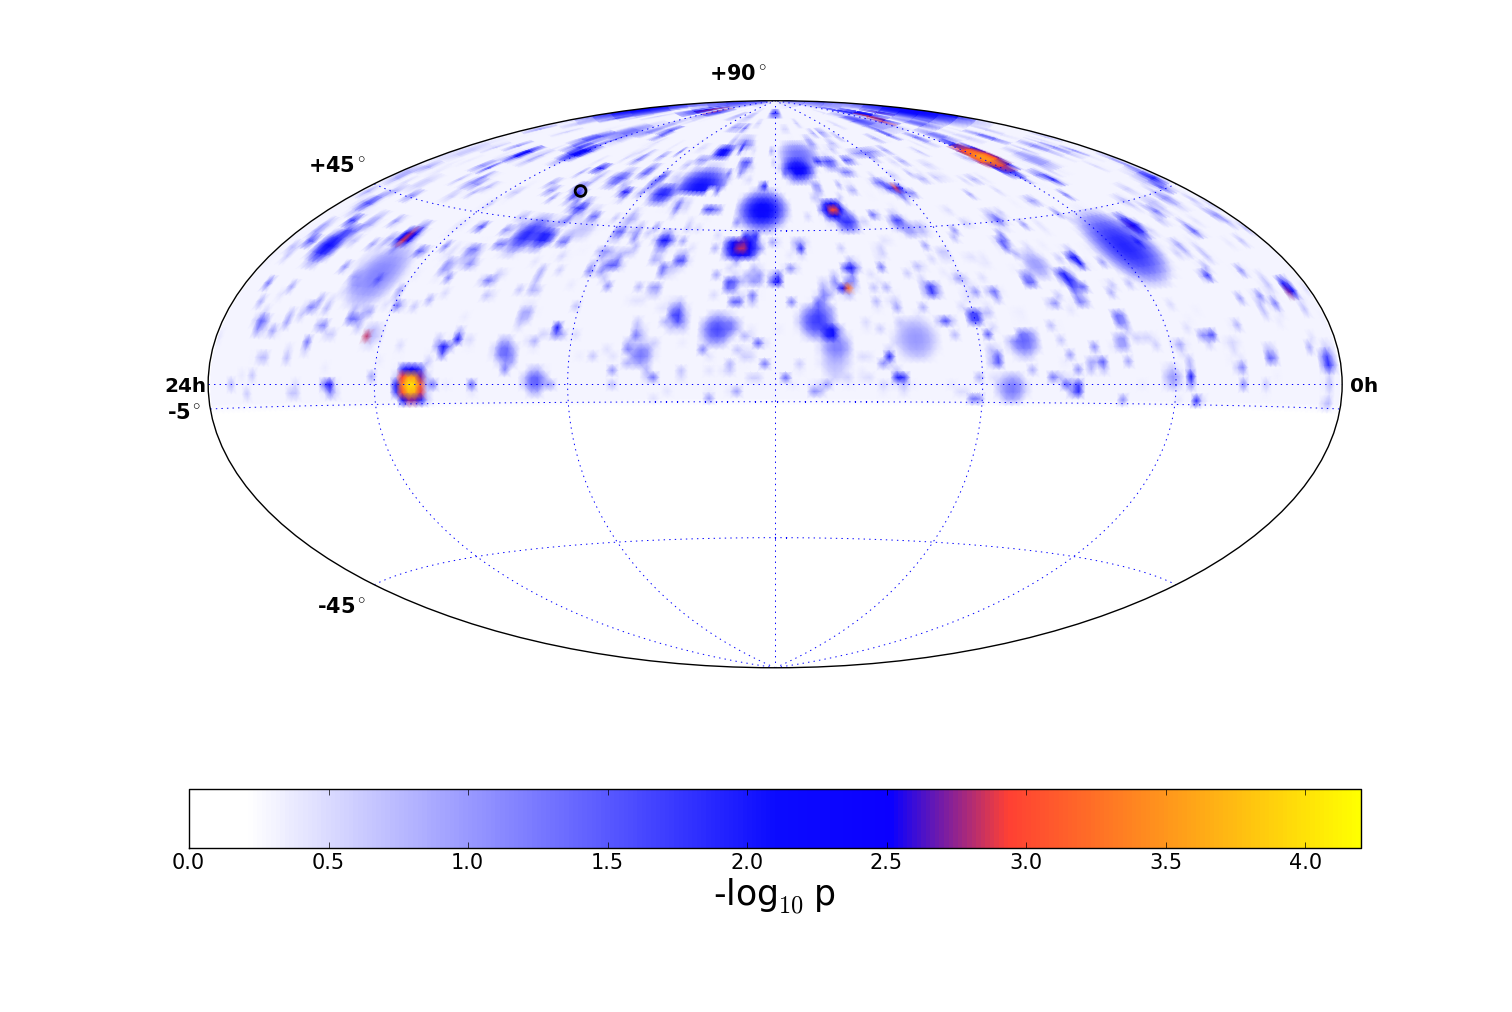
\includegraphics[width=1.0\textwidth,keepaspectratio]{plots/RealResultSkyMap.png}
  \end{center}
  \caption[Results Sky Map]{Sky map of pre-trials p-values for best fit flares per bin. The black circle identifies the location of the most significant flare found at RA = 268.75$^\circ$ and Declination = 54.25$^\circ$.}
  \label{fig:RealSkyMap}
\end{figure}


%% In a manner similar to \objectname authors can provide links to dataset
%% hosted at participating data centers via the \dataset{} command.  The
%% second curly bracket argument is printed in the text while the first
%% parentheses argument serves as the valid data set identifier.  Large
%% lists of data set are best provided in a table (see Table 3 for an example).
%% Valid data set identifiers should be obtained from the data center that
%% is currently hosting the data.
%%
%% Note that AASTeX interprets everything between the curly braces in the 
%% macro as regular text, so any special characters, e.g. "#" or "_," must be 
%% preceded by a backslash. Otherwise, you will get a LaTeX error when you 
%% compile your manuscript.  Special characters do not 
%% need to be escaped in the optional, square-bracket argument.

%% In this section, we use  the \subsection command to set off
%% a subsection.  \footnote is used to insert a footnote to the text.

%% Observe the use of the LaTeX \label
%% command after the \subsection to give a symbolic KEY to the
%% subsection for cross-referencing in a \ref command.
%% You can use LaTeX's \ref and \label commands to keep track of
%% cross-references to sections, equations, tables, and figures.
%% That way, if you change the order of any elements, LaTeX will
%% automatically renumber them.

%% This section also includes several of the displayed math environments
%% mentioned in the Author Guide.

%% The equation environment wil produce a numbered display equation.

%% The \notetoeditor{TEXT} command allows the author to communicate
%% information to the copy editor.  This information will appear as a
%% footnote on the printed copy for the manuscript style file.  Nothing will
%% appear on the printed copy if the preprint or
%% preprint2 style files are used.

%% The eqnarray environment produces multi-line display math. The end of
%% each line is marked with a \\. Lines will be numbered unless the \\
%% is preceded by a \nonumber command.
%% Alignment points are marked by ampersands (&). There should be two
%% ampersands (&) per line.

%% If you wish to include an acknowledgments section in your paper,
%% separate it off from the body of the text using the \acknowledgments
%% command.

%% Included in this acknowledgments section are examples of the
%% AASTeX hypertext markup commands. Use \url without the optional [HREF]
%% argument when you want to print the url directly in the text. Otherwise,
%% use either \url or \anchor, with the HREF as the first argument and the
%% text to be printed in the second.

\acknowledgments



%% To help institutions obtain information on the effectiveness of their
%% telescopes, the AAS Journals has created a group of keywords for telescope
%% facilities. A common set of keywords will make these types of searches
%% significantly easier and more accurate. In addition, they will also be
%% useful in linking papers together which utilize the same telescopes
%% within the framework of the National Virtual Observatory.
%% See the AASTeX Web site at http://aastex.aas.org/
%% for information on obtaining the facility keywords.

%% After the acknowledgments section, use the following syntax and the
%% \facility{} macro to list the keywords of facilities used in the research
%% for the paper.  Each keyword will be checked against the master list during
%% copy editing.  Individual instruments or configurations can be provided 
%% in parentheses, after the keyword, but they will not be verified.


%% Appendix material should be preceded with a single \appendix command.
%% There should be a \section command for each appendix. Mark appendix
%% subsections with the same markup you use in the main body of the paper.

%% Each Appendix (indicated with \section) will be lettered A, B, C, etc.
%% The equation counter will reset when it encounters the \appendix
%% command and will number appendix equations (A1), (A2), etc.


%% The reference list follows the main body and any appendices.
%% Use LaTeX's thebibliography environment to mark up your reference list.
%% Note \begin{thebibliography} is followed by an empty set of
%% curly braces.  If you forget this, LaTeX will generate the error
%% "Perhaps a missing \item?".
%%
%% thebibliography produces citations in the text using \bibitem-\cite
%% cross-referencing. Each reference is preceded by a
%% \bibitem command that defines in curly braces the KEY that corresponds
%% to the KEY in the \cite commands (see the first section above).
%% Make sure that you provide a unique KEY for every \bibitem or else the
%% paper will not LaTeX. The square brackets should contain
%% the citation text that LaTeX will insert in
%% place of the \cite commands.

%% We have used macros to produce journal name abbreviations.
%% AASTeX provides a number of these for the more frequently-cited journals.
%% See the Author Guide for a list of them.

%% Note that the style of the \bibitem labels (in []) is slightly
%% different from previous examples.  The natbib system solves a host
%% of citation expression problems, but it is necessary to clearly
%% delimit the year from the author name used in the citation.
%% See the natbib documentation for more details and options.

\bibliography{IceCube_2012_ChkGRB_Limits}{}

\clearpage

%% Use the figure environment and \plotone or \plottwo to include
%% figures and captions in your electronic submission.
%% To embed the sample graphics in
%% the file, uncomment the \plotone, \plottwo, and
%% \includegraphics commands
%%
%% If you need a layout that cannot be achieved with \plotone or
%% \plottwo, you can invoke the graphicx package directly with the
%% \includegraphics command or use \plotfiddle. For more information,
%% please see the tutorial on "Using Electronic Art with AASTeX" in the
%% documentation section at the AASTeX Web site, http://aastex.aas.org/
%%
%% The examples below also include sample markup for submission of
%% supplemental electronic materials. As always, be sure to check
%% the instructions to authors for the journal you are submitting to
%% for specific submissions guidelines as they vary from
%% journal to journal.

%% This example uses \plotone to include an EPS file scaled to
%% 80% of its natural size with \epsscale. Its caption
%% has been written to indicate that additional figure parts will be
%% available in the electronic journal.

%\begin{figure}
%\epsscale{.80}
%\plotone{f1.eps}
%\caption{Derived spectra for 3C138 \citep[see][]{heiles03}. Plots for all %sources are available
%in the electronic edition of {\it The Astrophysical Journal}.\label{fig1}}
%\end{figure}

\clearpage

%% Here we use \plottwo to present two versions of the same figure,
%% one in black and white for print the other in RGB color
%% for online presentation. Note that the caption indicates
%% that a color version of the figure will be available online.
%%

%\begin{figure}
%\plottwo{f2.eps}{f2_color.eps}
%\caption{A panel taken from Figure 2 of \citet{rudnick03}. 
%See the electronic edition of the Journal for a color version 
%of this figure.\label{fig2}}
%\end{figure}

%% This figure uses \includegraphics to scale and rotate the still frame
%% for an mpeg animation.

%\begin{figure}
%\includegraphics[angle=90,scale=.50]{f3.eps}
%\caption{Animation still frame taken from \citet{kim03}.
%This figure is also available as an mpeg
%animation in the electronic edition of the
%{\it Astrophysical Journal}.}
%\end{figure}

%% If you are not including electonic art with your submission, you may
%% mark up your captions using the \figcaption command. See the
%% User Guide for details.
%%
%% No more than seven \figcaption commands are allowed per page,
%% so if you have more than seven captions, insert a \clearpage
%% after every seventh one.

%% Tables should be submitted one per page, so put a \clearpage before
%% each one.

%% Two options are available to the author for producing tables:  the
%% deluxetable environment provided by the AASTeX package or the LaTeX
%% table environment.  Use of deluxetable is preferred.
%%

%% Three table samples follow, two marked up in the deluxetable environment,
%% one marked up as a LaTeX table.

%% In this first example, note that the \tabletypesize{}
%% command has been used to reduce the font size of the table.
%% We also use the \rotate command to rotate the table to
%% landscape orientation since it is very wide even at the
%% reduced font size.
%%
%% Note also that the \label command needs to be placed
%% inside the \tablecaption.

%% This table also includes a table comment indicating that the full
%% version will be available in machine-readable format in the electronic
%% edition.

\clearpage


\end{document}

%%
%% End of file `sample.tex'.
